\chapter{Ergebnisse}
\section{Berechnung von SHAP-Werten}

TODO: Berechnung der SHAP-Werte.

\section{Interpretation}

TODO: Analyse der Ergebnisse, Interpretation von SHAP-Werten, Vergleich der Koeffizienten mit den \acs{SHAP-Werten}.

\subsection{Lokale Interpretation}

\begin{figure}[h]
    \caption{SHAP Summary Plot}
    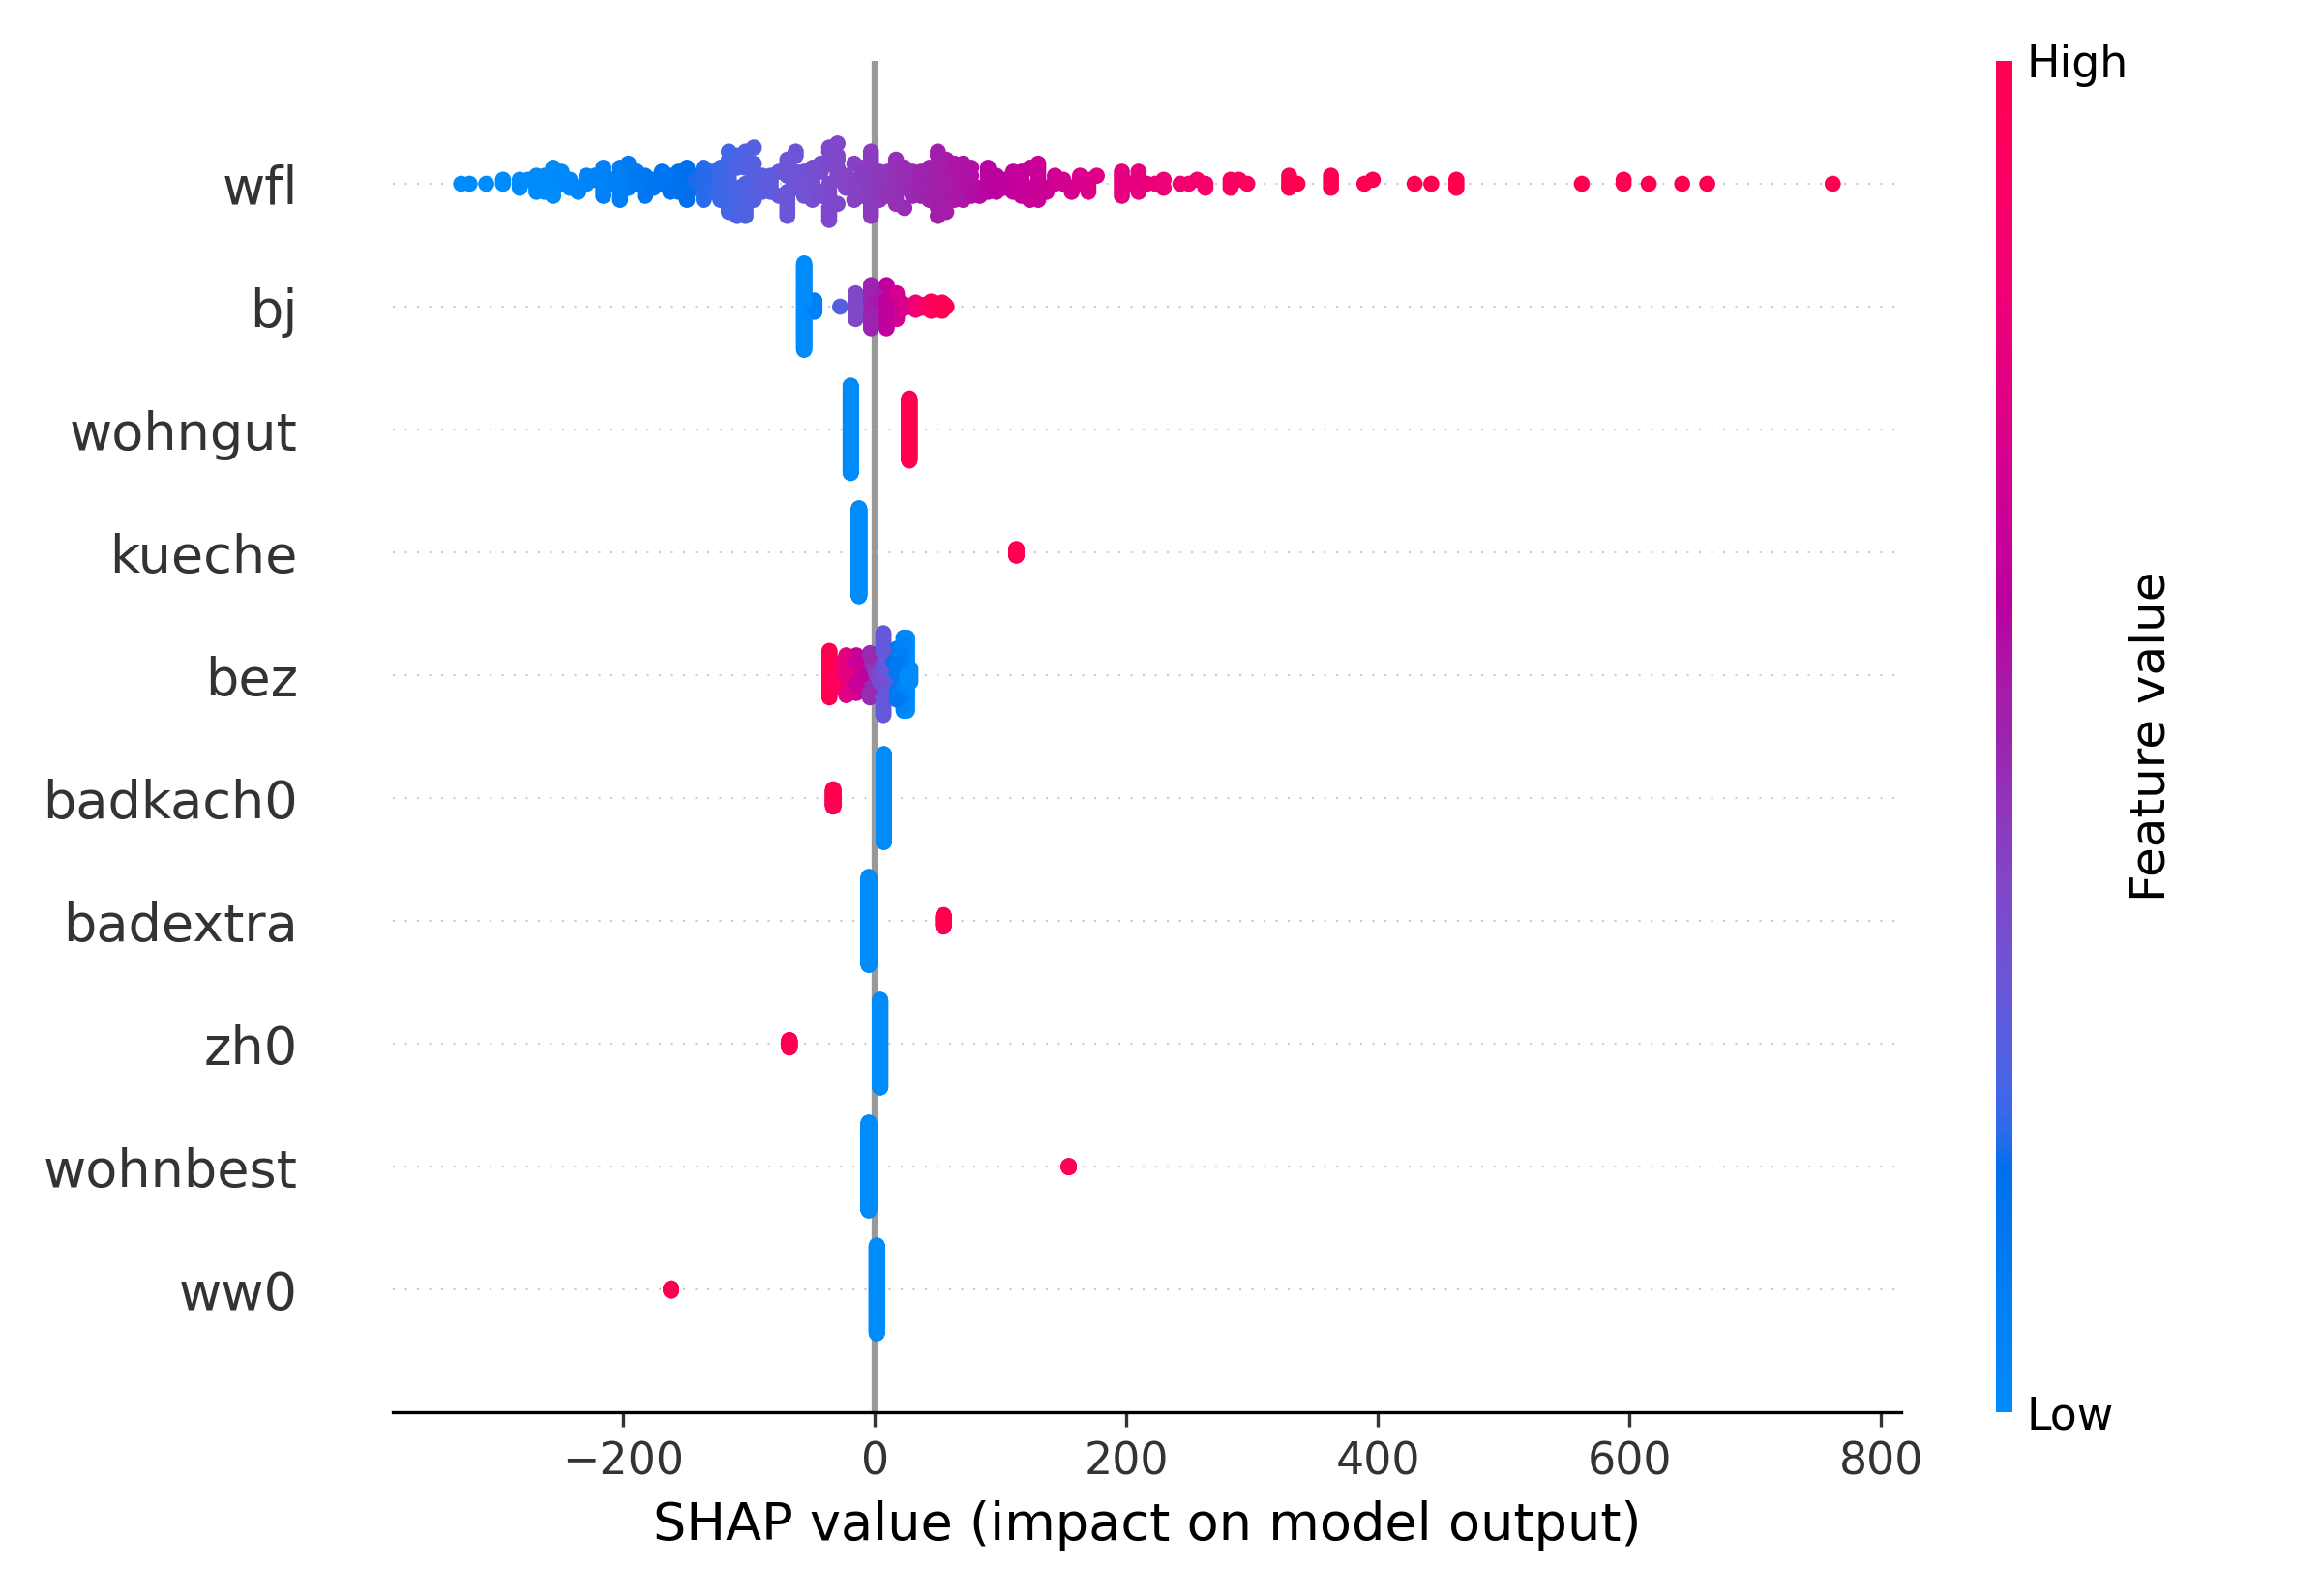
\includegraphics[width=1\textwidth]{../scripts/images/shap_summary_plot.png}
    Quelle: Eigene Darstellung, \ref{linreg}.
    \label{pic:shap_summary}
\end{figure}


\subsection{Globale Interpretation}

\begin{figure}[h]
    \caption{SHAP Bar Plot}
    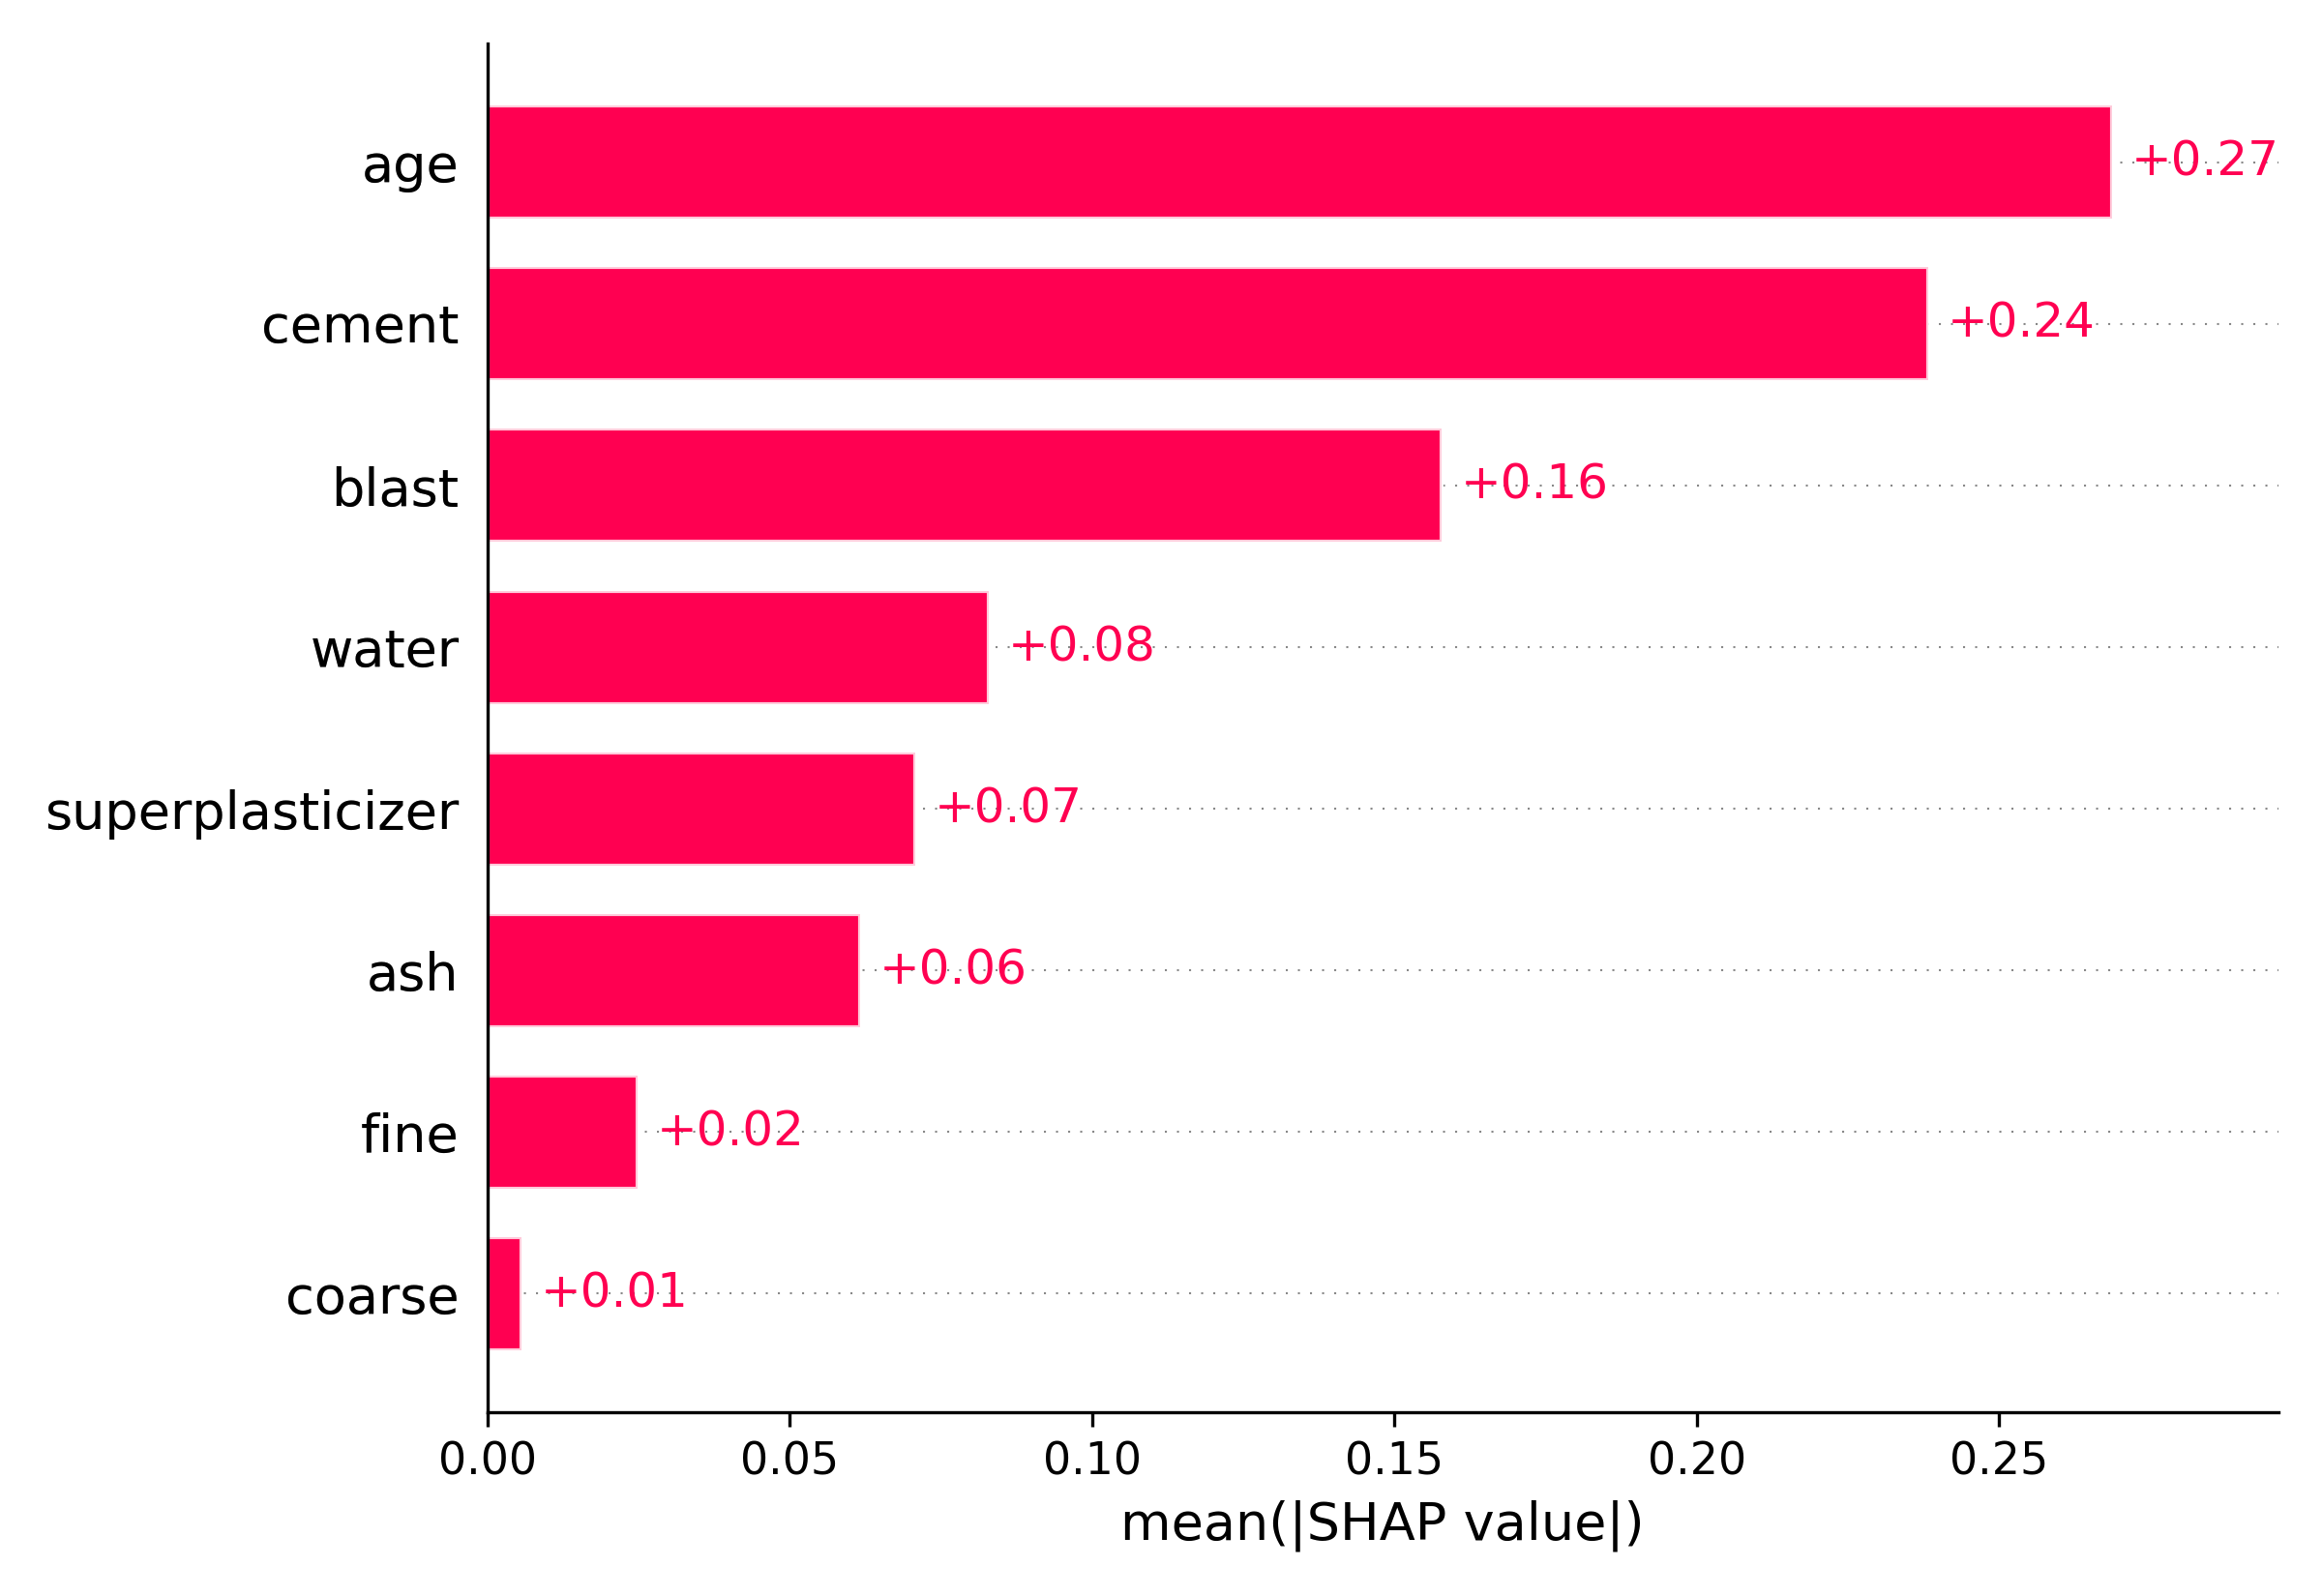
\includegraphics[width=1\textwidth]{../scripts/images/shap_bar_plot.png}
    Quelle: Eigene Darstellung, \ref{linreg}.
    \label{pic:shap_bar}
\end{figure}

\begin{figure}[h]
    \caption{SHAP Waterfall Plot}
    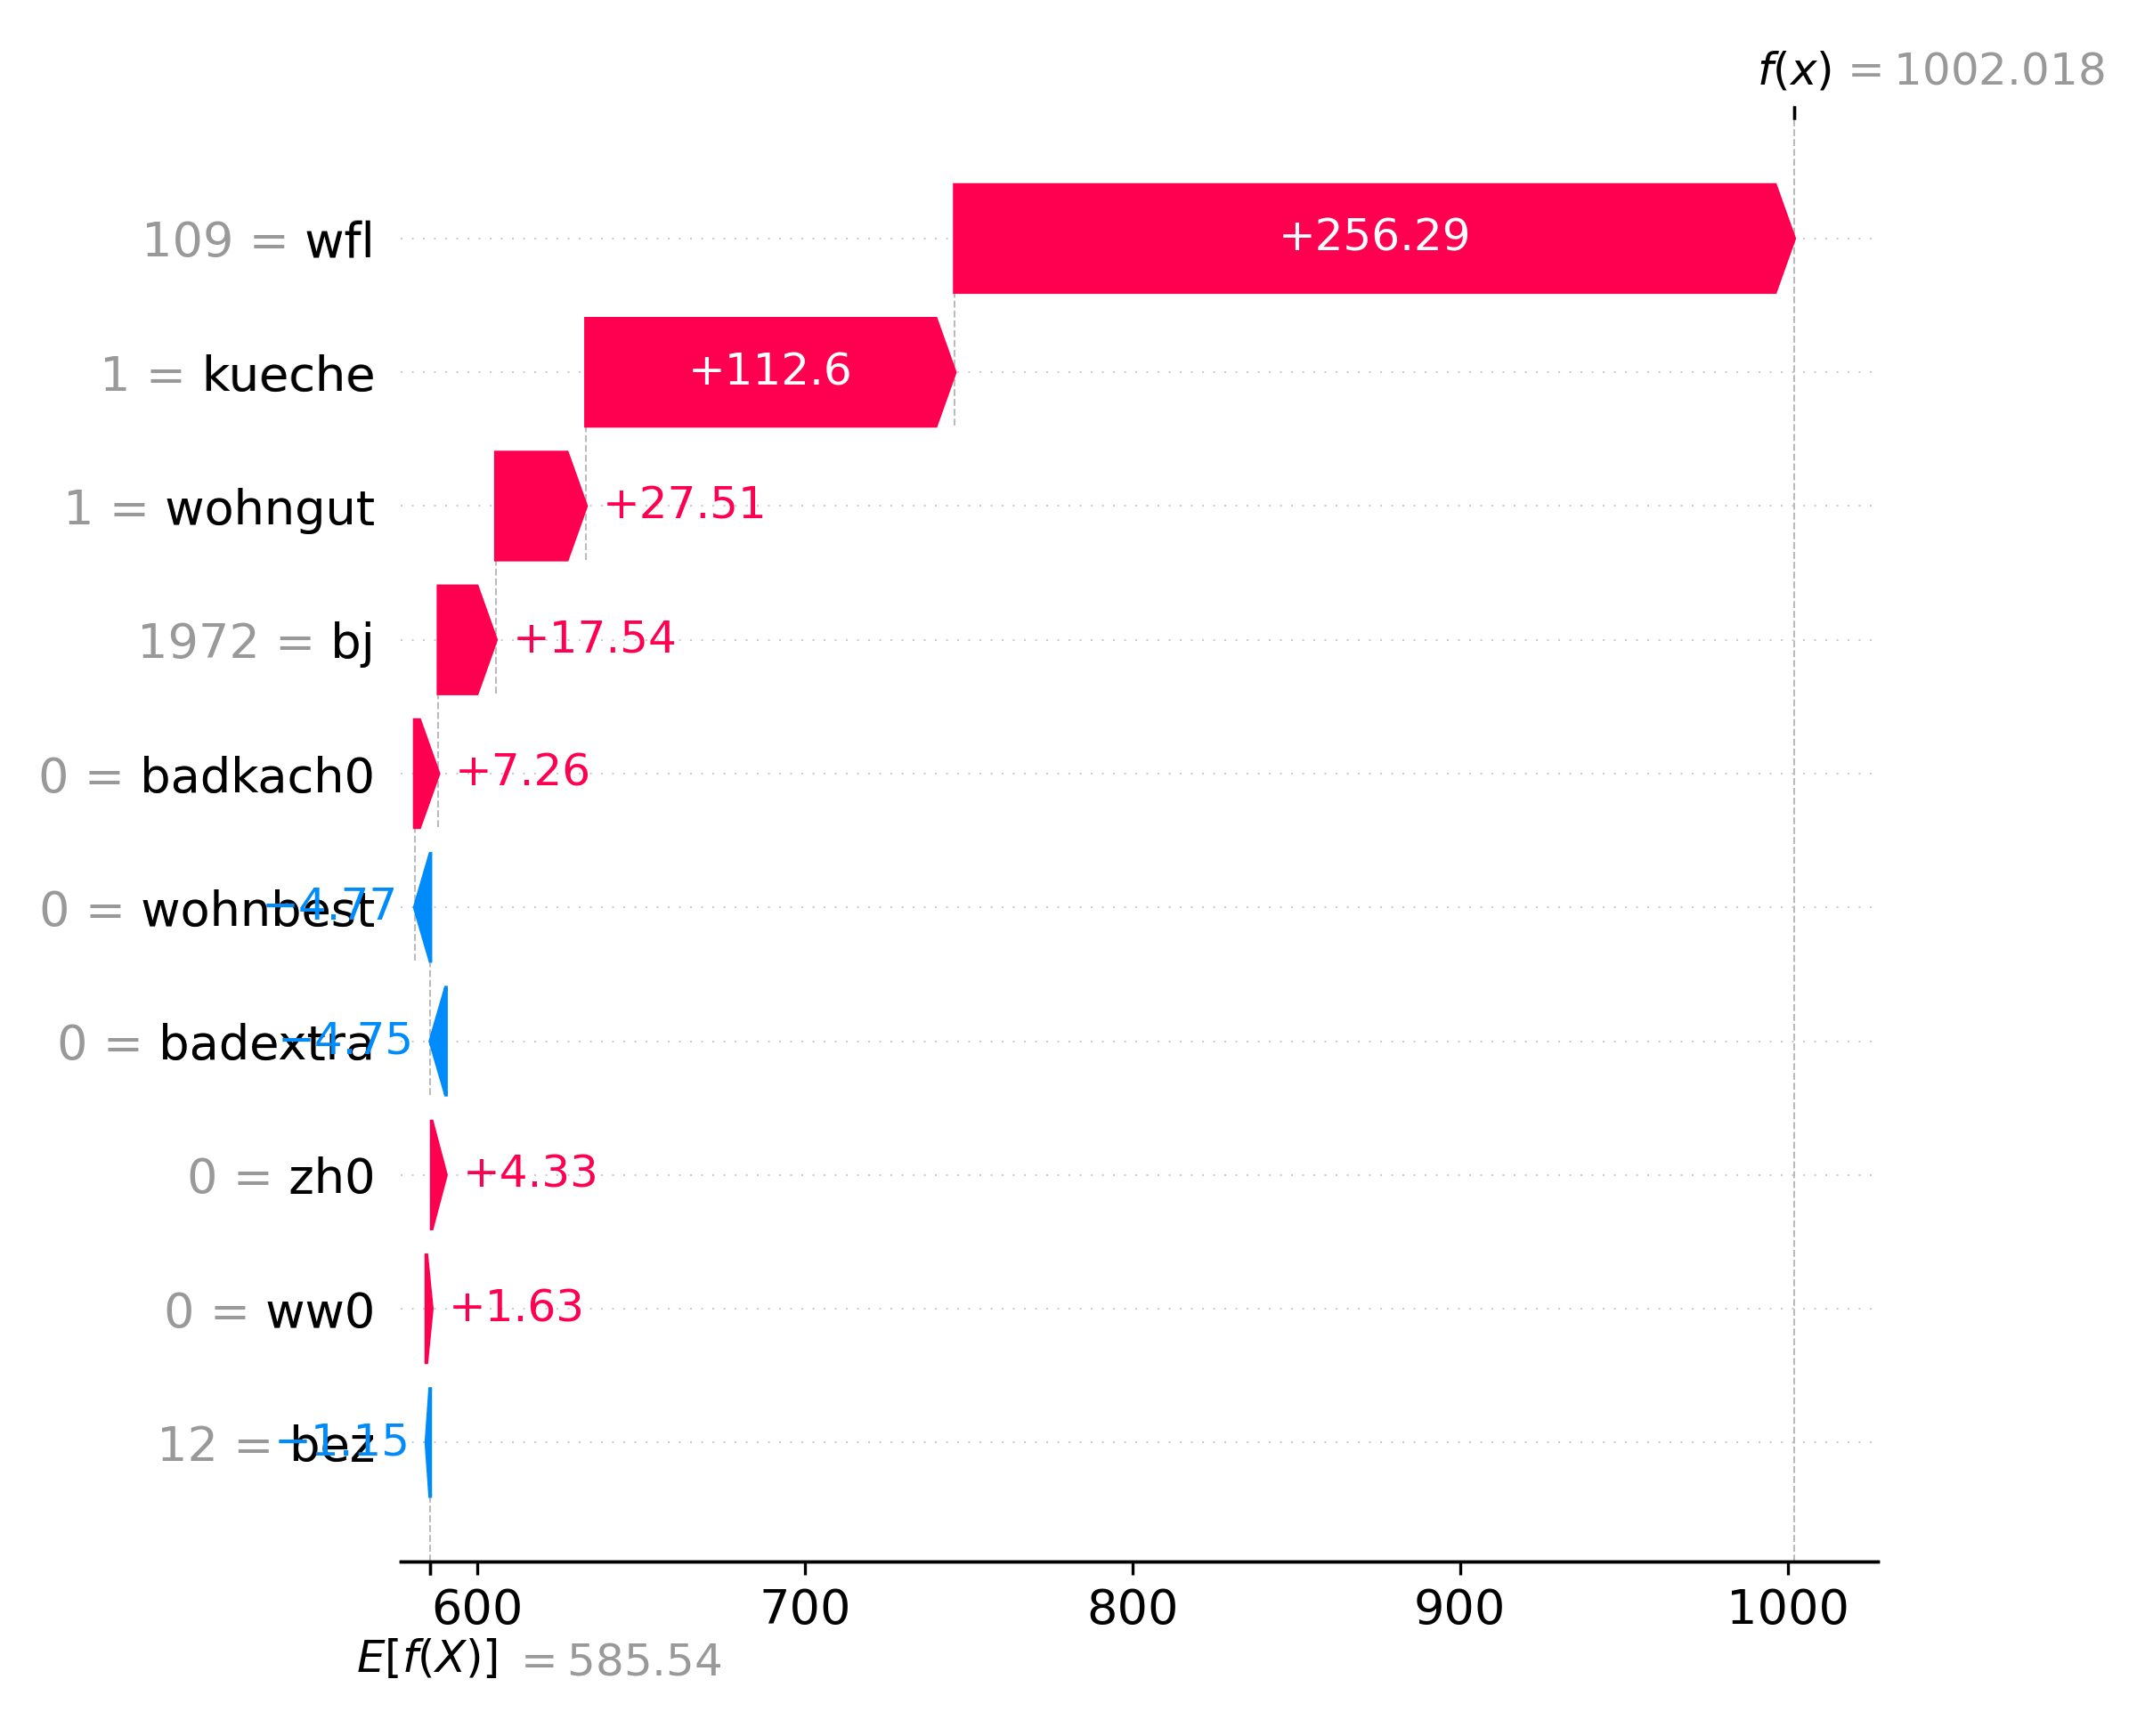
\includegraphics[width=1\textwidth]{../scripts/images/shap_waterfall_plot.png}
    Quelle: Eigene Darstellung, \ref{linreg}.
    \label{pic:shap_waterfall}
\end{figure}